\begin{table}
\caption{Nomenclature and abbreviations used in the manuscript \label{tab:symabbr}}
\centering
\begin{tabular}{|p{1.3cm}@{\extracolsep{\fill}}p{7.8cm} @{\extracolsep{\fill}}p{1.3cm}@{\extracolsep{\fill}}p{5.6cm}|}\hline
\multicolumn{2}{|l}{ \textbf {Nomenclature}}  & \multicolumn{2}{l|}{\textbf {Abbreviations}} \\[5pt]
$\mathbf{A}$     & Adjacency matrix                                                               &   ACF     & auto-correlation function \\ 
$b_p$                & betweenness centrality of vertex $p$                                &  AR	&	auto regressive 	 \\
$c_{p}$              & closeness centrality of vertex $p$                                     &  B. P.  &	 before present \\
$\mathcal{C}$    & global clustering coefficient 						  &   COPTN &	 cross ordinal pattern transition network \\
$\mathcal{C}_{p}$    & local clustering coefficient of vertex $p$ 			 &   CRP	&	cross recurrence plots	\\
$\mathcal{D}$    	& network diameter							& 	DVG	& difference visibility graph \\
$\hat{D}_{\mathcal{C}} $              &      clustering dimension			&	ER        & Erd\"os R\'enyi random network  \\
$\hat{D}_{\mathcal{T}} $              &      transitivity dimension			&	fBm       & fractional Brownian motion  \\
$\Delta k_p$    & excess degree of vertex $p$						&	fGn        & fractional Gaussian noise \\
$\Delta_{rel} k_p$    & relative excess degree of vertex $p$			&	FNN      & false nearest neighbors\\
$\Delta t $         & sampling time  								 &   GS        & generalized synchronization \\
$\delta(\cdot)$   & delta function ($\delta(x) = \{ 1 | x = 0; 0 | x \neq = 0 \}$)  &  HVG      & horizontal visibility graph\\
$\varepsilon$    & radius of neighborhood							  &  IRN	&	inter-system recurrence network  \\
$e_p$       & local efficiency of vertex $p$ 							  &  ISN   &	international sunspot number \\
$E$   	 & edge set										&   JOPTN  &	 joint ordinal pattern transition network  \\
$\mathcal{E}$    & global efficiency 								 &  JRN	&	joint recurrence network	 \\
$F(k)$   &  cumulative degree distribution function 		 			&   KLD	  & Kullback-Leibler divergence  \\
$GIC$   & graph index complexity								&	KS  		 & Kolmogorov-Smirnov test	\\
$\gamma$   	 & power law exponent							&	LIA     & 	little ice age \\
$H$   	 & Hurst exponent									&	LPVG & limited penetration visibility graph\\
$k_p$       & degree of vertex $p$  								  &  Ma    &	  million years \\
$l_{pq}$              & shortest path between vertices $p$ and $q$                    &  ODP  &	 ocean drilling program \\
 $\mathcal{L}$      & average path length 							&    OP        & ordinal pattern \\
$\lambda$     & Lyapunov exponent; exponential scaling factor  		&   OPTN	&   ordinal pattern transition network \\
$m$        & embedding dimension 								  & PDF      & probability density function  \\
$\mu$    & coupling strength									&	PS        & phase synchronization  \\
$N$      & length of time series 									&     RGG &	random geometric graph 	 \\
$\pi$               & ordinal pattern 			 						  & RN       & recurrence network   \\
$p(x) $              & probability density function of $x$ 					  &  RP        & recurrence plot  \\
$RR$    & recurrence rate 										& 	RQA      & recurrence quantification analysis  \\
$\mathcal{R}$      & assortativity coefficient 						&    SF         & scale free  \\
$r$			&	cross correlation coefficient 					&	SSA	  &  sunspot area\\
$\rho $              &      edge (link) density of a network 				&	SSN      & sunspot numbers \\
$\sigma_{pq}$     & multiple shortest paths between vertices $p$ and $q$        & SW        & small world\\
$\tau$      & embedding delay 									  &     UPO      & unstable periodic orbits\\
$\mathcal{T}$    & transitivity									&	VG        & visibility graph \\
$S$    	& Shannon entropy									&	&	\\
$\Theta(\cdot)$   	 & Heaviside function 						&	&	 \\
$\mathbf{W}$    	& weighted adjacency matrix 					&	 &	 \\
$\Omega$    & average frequency			 					&	&	\\
$w_{pq}$   	      &       transition frequency from vertex $p$ to $q$		&	&	 \\
$\hat{x}$   	 &       estimator of $x$							&	&	 \\
$\left< x \right> $   	 &       average of $x$						&	&	 \\
$V$    	& vertex set										&	 &	\\
\hline
\end{tabular}
\end{table}

\clearpage


\section{Introduction}
Artificial Intelligence is generating data in new forms of complexity, leading to the new era of big data \cite{schonberger2013}. This brings big challenges for researchers from various fields working together to extract patterns or new structures from data of very high volume, high velocity, or high variety. Advanced interdisciplinary data analytics techniques help to capture the hidden structures amidst otherwise chaotic data points, including approaches from machine learning, data mining, statistics, natural language and text processing \cite{hurwitz2018}. In consequence, we transform the messy datasets into something that we can learn fast, which allows us making better and faster decisions. Among these processes, there is ample scope for developing new tools for data analysis. In the context of dynamical systems and statistical physics, such methods are often associated with concepts like complex networks \cite{Albert2002,Newman2003,Newmanbook2010} and complexity theory. 

In this report, we focus on some particular subfield that has attracted great interest in the last years -- the application of various approaches from complex network theory in the context of nonlinear time series analysis \cite{kantz1997,abarbanel1993,Sprott2003}. A time series is a sequence of data points indexed by the time of observations, which are made at successive, in many cases equally spaced points in time. Hence, time series data have a natural discrete temporal ordering. Examples of such time series cover a great variety of variables potentially relevant for everyday life, including (but not being limited to) the following areas: (i) weather conditions, like surface-air temperatures, sea level pressure, and wind speeds that are collected from meteorological stations or satellites; (ii) finance, e.g., the daily closing prices of stock market indices like
the Dow Jone Industrial Average, individual assets, or exchange rates; (iii) bio-medical conditions of humans, for instance, physiological and clinical data that are collected by electroencephalogram (EEG) monitoring or high resolution brain imaging techniques like magnetic resonance imaging (MRI) and computed tomography (CT). Time series analysis considers the study of the entire collection of observations as a whole instead of individual numerical values at several temporal instances. 

The natural temporal ordering makes time series analysis distinct from data analysis in the case of no natural ordering of the observations (for instance, cross-sectional studies of explaining people's wages by reference to their respective education levels, or spatial data analysis accounting for house prices by the location as well as the intrinsic characteristics of the houses). In order to discover hidden patterns of such more general large data sets from different sources, data mining tools have been proposed in the research field of computer science, which have also found many applications in the context of time series mining \cite{Keogh2003,FU2011,Aghabozorgi2015}. Here, time series mining focuses more on indexing, clustering, classification, segmentation, motif discovery, and forecasting \cite{Keogh2003,Aghabozorgi2015}. In the recent decade, there has been a considerable amount of rapid developments of data mining tools initiated by the advent of big data and cloud computing reflecting the increasing size and complexity of available datasets. One particular example of such developments is to design algorithms of high efficiency that can learn from and make predictions on the large data sets in terms of supervised or unsupervised learning methods \cite{hurwitz2018}. Furthermore, there is an emerging trend to combine complex network approaches with data mining tools, which provide many novel analysis concepts for discovering hidden pattern in large data sets \cite{Zanin2016}. The classification task of data mining allows for a rich representation of some complex systems, for instance, a meaningful reconstruction of functional networks from rather large data sets by choosing feature vectors of lower dimension \cite{Zanin2014a}. Hence, the application of feature selection algorithms provides a complementary understanding of the characteristics of network structures. There have been a few successful applications of mining tools for complex network analysis from synthetic and experimental data, in particular, related with disease classification \cite{Zanin2014a,Karsakov2017,Whitwell2018}. 

Despite the considerable practical relevance of time series mining algorithms, there has been practically no overlap with the subject of nonlinear time series analysis by means of complex network methods, which is the focus of this report. Unlike most established data mining techniques, the time series network approaches reviewed here are based on the dynamical systems theory \cite{Ott1993,kantz1997} and present themselves as state-of-the-art contributions to nonlinear time series analysis \cite{Bradley2015c}. From the viewpoint of complex network research, the topics reviewed in this paper can be regarded as successful applications of network theory to tackling synthetic as well as experimental series from a diversity of fields of applications. We will discuss potential generalizations of the different time series network approaches in the context of data mining tools wherever appropriate.
 
	\subsection{Nonlinear time series analysis}
	Time series analysis is essentially data compression \cite{Bradley2015c}. Given a time series, we interpret the underlying dynamical system by a few characteristic numbers that are computed from a large sample of measurements. Therefore, the reduced information as represented by these characteristic numbers must highlight some specific features of the system. Early approaches of time series analysis heavily relied on the linearity assumption on the underlying processes, for instance, autoregressive (AR) and moving average (MA) models, both of which result in almost exponentially decaying auto-correlation functions. However, it is by now well accepted that the dynamical laws governing nature or human activities are seldomly linear. Nonlinearity is everywhere, for example: (a) phase transitions (e.g., the melting of the ice of a glacier) are an important signature of nonlinearity in physical systems; (b) animals behave differently (e.g. hunting effort) during times of short food supply versus times of abundant food supply; (c) for many electronic devices (e.g., transistors) saturation velocity and current are well-known nonlinear phenomena; (d) in many engineering problems, controlling the system to operate at desired states introduces various forms of feedback mechanisms. Accordingly, the development of nonlinear time series analysis has been primarily driven by the needs to overcome the corresponding limitations of linear models and methods. 

	Nonlinear time series analysis is not as well established and far less well understood than its linear counterpart \cite{kantz1997}. The collection of ideas and techniques of nonlinear time series analysis originates from the fast development of dynamical systems theory or so-called ``chaos theory'', which explores system dynamics by a set of nonlinear difference equations or nonlinear ordinary differential equations. Techniques from chaos theory allow to characterize dynamical systems in which nonlinearities give rise to a complex temporal evolution, for instance, a sensitive dependence on initial conditions and strongly limited predictability. Importantly, this concept allows extracting information that cannot be resolved using classical linear techniques such as the power spectrum or spectral coherence.

	Since its early stages in the 1980s \cite{Packard1980}, numerous conceptual approaches have been introduced for studying the characteristic features of nonlinear dynamical systems based on observational time series \cite{abarbanel1993,kantz1997,Sprott2003}. The mathematical beauty of this analysis framework is that we characterize the invariant measure in phase space in a number of different ways. Generally speaking, we quantify the system from either geometric or dynamic perspectives. Important examples include, but are not limited to the correlation dimension (or, more generally, the spectrum of generalized fractal dimensions $D_q$ \cite{Grassberger1983PRL}) that has been suggested to characterize the geometry of chaotic attractors in phase space; the Lyapunov exponent as a measure for stability of dynamics with respect to infinitesimal perturbations; and the Kolmogorov-Sinai entropy (or other information theory measures) to quantify uncertainty about the future states of a chaotic trajectory. All these techniques have in common that they quantify certain dynamically invariant phase space properties of the considered system based on temporally discretized realizations of individual trajectories. 

	One typical task is to perform a precise system characterization from a single time series, which is, however, not the final goal of most time series analyses \cite{Bradley2015c}. Here, we give just a few examples that nonlinear time series analysis can contribute to: (1) system characterization from a single time series; (2) discrimination between a signal and some other signals; (3) quantification of various bifurcation transition scenarios to complex dynamics, including period doubling, band merging, more general examples of subtle changes like intermittency or other phenomena associated with chaos-to-chaos transitions, detection of general regime shifts or tipping points in essential dynamical properties; (4) testing for time series reversibility; (5) noise reduction and filtering; and (6) prediction of future time series values.

	The aforementioned nonlinear time series characteristics are based on univariate series, i.e., they can be applied to single signals measured upon individual dynamical systems. In contrast, bivariate measures are used to analyze pairs of signals measured simultaneously from two dynamical systems. There has been considerable interest in the study of the synchronization behavior of coupled chaotic systems, which have been observed in many physical and biological systems \cite{Boccaletti2002,Pikovsky_Kurths_synchr}. Thus, such bivariate time series analysis measures aim to detect and to distinguish transition forms from non-synchronized states to synchronization (for instance, paths to phase synchronization, lag synchronization, complete synchronization and generalized synchronization). In different synchronization scenarios, it is important to extract not only the coupling strength but also the direction of these couplings, i.e., identifying causal relationships between the studied sub-systems. Unraveling the governing functional interactions between sub-systems contained in a large network of complex connectivity topology remains a big challenge in modern nonlinear sciences \cite{Boccaletti2006,Stankovski2017}. Various methods have been proposed to extract the statistical associations from data, for instance, Pearson correlation, mutual information (including its time delayed version) \cite{Frenzel_prl_2007,vejmelka_pre_2008}, Granger causality \cite{Granger_1969,Dhamala_prl2008}, transfer entropy \cite{schreiber_prl2000,runge2012}, or methods for detecting coupling directions from time series data \cite{Quiroga_pre2000,Rosenblum2001,rosenblum_pre2002,smirnov_pre2005,Palus_pre_2007,Romano_pre_2007,bahraminasab_prl2008,Nawrath_prl_2010}. More generally, coupling functions can have various forms. We do not expand the corresponding discussion here, but refer the interested readers to several review papers on this topic \cite{Ding_Book_2007,Hlavackovaschindler2007,Stankovski2017}.

	Nonlinear time series analysis provides a powerful toolbox of methods that are useful for many applications, but also have some practical limitations. Some common problems originating from experimental measurements challenge the computations of nonlinear measures. For instance, most of the existing nonlinear methods are in practice only applicable to low-dimensional dynamical systems. In reality, very few real-world data sets are measured by perfect sensors operating on low-dimensional dynamics. One has to be aware of non-stationarity, proper choice of embedding parameters, dependence on finite data length (with possibly rather short time series in many real-world situations), effects of noise, or irregular sampling \cite{Bradley2015c}. Statistical concerns come also from algorithmic aspects requiring proper choice of parameters. For instance, scaling regimes should be pronounced for implementing linear line fitting to estimate the numerical values of dynamically invariant measures like fractal dimensions and Lyapunov exponents, the proper selection of which often influences the results significantly. In addition, computational complexity has to be well evaluated since it varies significantly among these measures. Currently, the choice of algorithmic parameters largely depends on the researchers' experience. 

	In this review, we demonstrate that complex network approaches can contribute many aspects that we have discussed above for nonlinear time series analysis. More importantly, complex network approaches can solve partially some fundamental and long standing problems not successfully addressed by other existing methods so far, yielding a more robust estimation of dynamical invariants, for instance, using the transitivity dimension and local clustering dimension of recurrence networks to approximate the fractal dimension of the system \cite{Donner2011b}; or by computing the mean out-degree of ordinal pattern transition networks or the associated network diameter performing similarly well as the Lyapunov exponent \cite{McCullough2015}. 
	
	\subsection{Complex network approaches}
	With the recent increase in available computational capacities and rising data volumes in various fields of science, complex networks have become an interesting and versatile tool for describing structural interdependencies between mutually interacting units \cite{Albert2002,Boccaletti2006,Costa2007,Newman2003}. Besides ``classical'' areas of research (such as sociology, transportation systems, computer sciences, or ecology), where these units are clearly (physically) identifiable, the success story of complex network theory has recently lead to a variety of ``non-conventional'' applications. 

	One important class of such non-traditional applications of complex network theory are \emph{functional networks}, where the considered connectivity does not necessarily refer to ``physical'' vertices and edges, but reflects statistical interrelationships between the dynamics exhibited by different parts of the system under study. The term ``functional'' was originally coined in neuroscientific applications, where contemporaneous neuronal activity in different brain areas is often recorded using a set of standardized EEG channels. These data can be used for studying statistical interrelationships between different brain regions when performing certain tasks, having the idea in mind that the functional connectivity reflected by the strongest statistical dependencies can be taken as a proxy for the large-scale anatomic connectivity of different brain regions \cite{Bullmore2009,Zhou2006,Zhou2007}. Similar approaches have been utilized for identifying dominant interaction patterns in other multivariate data sets, such as climate data \cite{Tsonis2004,Donges2009b,Donges2009a}.

	Besides functional networks derived from multivariate time series, there have been numerous efforts for utilizing complex network approaches for quantifying structural properties of individual time series. By means of complex network analysis, the first step is to find a proper network representation for time series, i.e., an algorithm defining what network vertices and network edges are. To this end, several approaches have been proposed \cite{Zhang2006,Xu2008,Lacasa2008,Marwan2009,Donner2010a,Donner2011,McCullough2015}. Based on these network representations, the rich toolbox of complex network measures \cite{Boccaletti2006,Costa2007,Newman2003} provides various quantities that can be used for characterizing the system's dynamical complexity from a complex network viewpoint and allow discriminating between different types of dynamics~\cite{Donner2011}. More importantly, complementary features of dynamical systems (i.e., properties that are not captured by existing methods of time series analysis) can be resolved. In this report, we give an exhaustive review on complex network approaches for nonlinear time series analysis. To this end, we first provide an overall impression of various complex network representations for time series, which are illustrated in Figs.~\ref{fig:lorenz_adj-matrices},\ref{fig:lorenz_network} for the $x$-coordinate of one realization of the Lorenz system (Eq.~\eqref{eqlorenz}) with the parameters $r=28$, $\sigma=10$ and $\beta=8/3$ (sampling time $\Delta t=0.02$). In the following sections, we will expand the discussions on the reconstruction of these networks from given time series data and their resulting characteristics. Specifically, we will focus on some important transformation methods that have been widely applied to various artificial as well as real-world observational or experimental data, in particular, recurrence networks, visibility graphs, and transition networks. In addition to these main approaches, we will also discuss some algorithmic variants of these concepts and corresponding relevant network measures wherever appropriate. 
\begin{figure}[htbp]
	\centering
	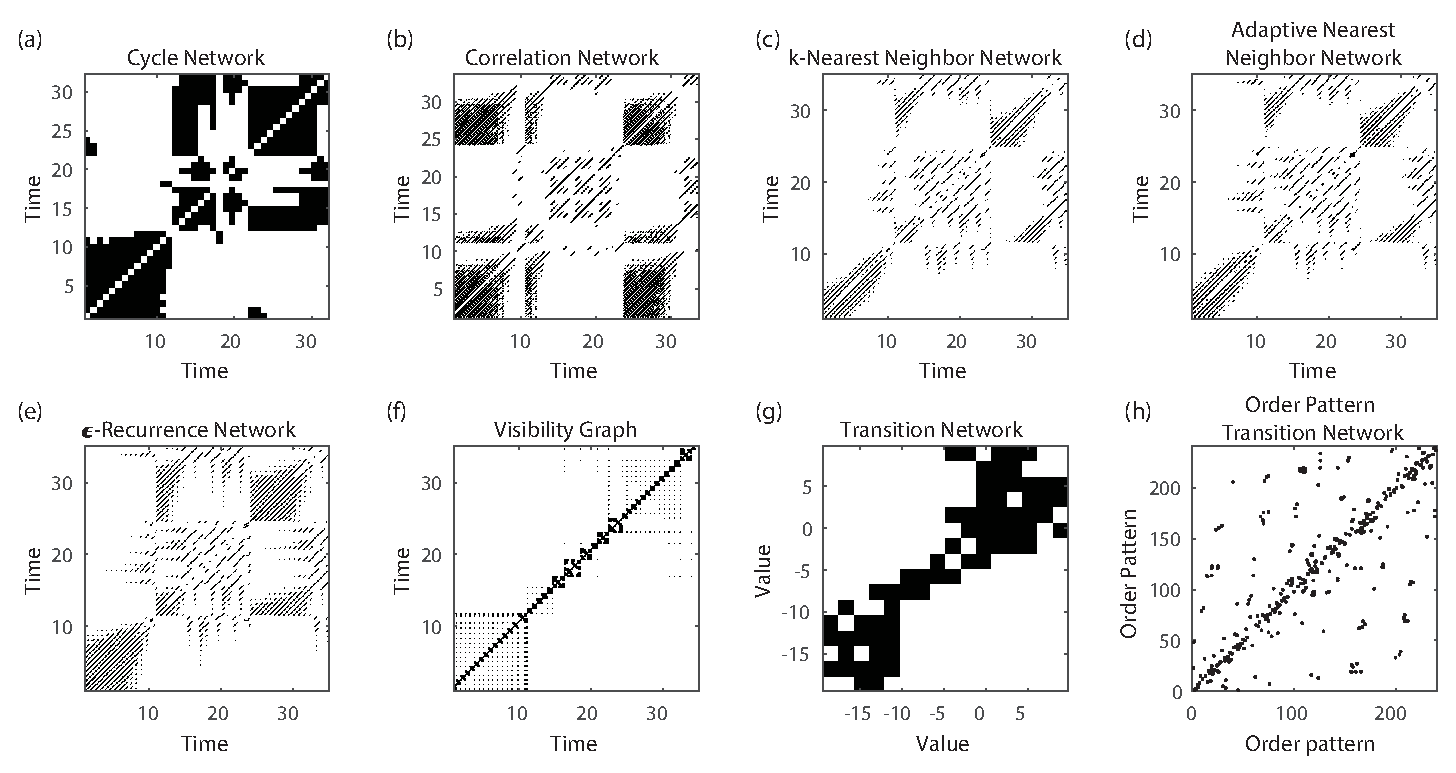
\includegraphics[width=\textwidth]{Chapter01_Introduction/lorenz_adj-matrix.eps} 
\caption{Adjacency matrices corresponding to different types of time series networks constructed from the $x$-coordinate of the Lorenz system: (a) cycle network ($N=40$, critical cycle distance in phase space $D_{max}=5$), (b) correlation network ($N=654$, embedding dimension $m=10$ with delay $\tau=3$), (c) $k$-nearest neighbor network {(asymmetric version)}, $N=675$, $m=3$, $\tau=3$, $k=10$, corresponding to a recurrence rate of $RR\approx 0.015$ using Euclidean norm, (d) adaptive nearest neighbor network $N=675$, $m=3$, $\tau=3$, (e) $\varepsilon$-recurrence network ($N=675$, $m=3$, $\tau=3$, $\varepsilon=2$, maximum norm), (f) visibility graph ($N=681$), and (g) coarse-graining based transition network (based on an equipartition of the range of observed values into $N=20$ classes of size $\Delta x=3.0$, minimum transition probability $p=0.2$ during 3 time steps), (h) ordinal pattern transition network ($N=240$ neglecting disconnected patterns, $m=6$, $\tau=3$). Modified from \cite{Donner2011}. } \label{fig:lorenz_adj-matrices}
\end{figure}
\begin{figure}[htbp]
	\centering
	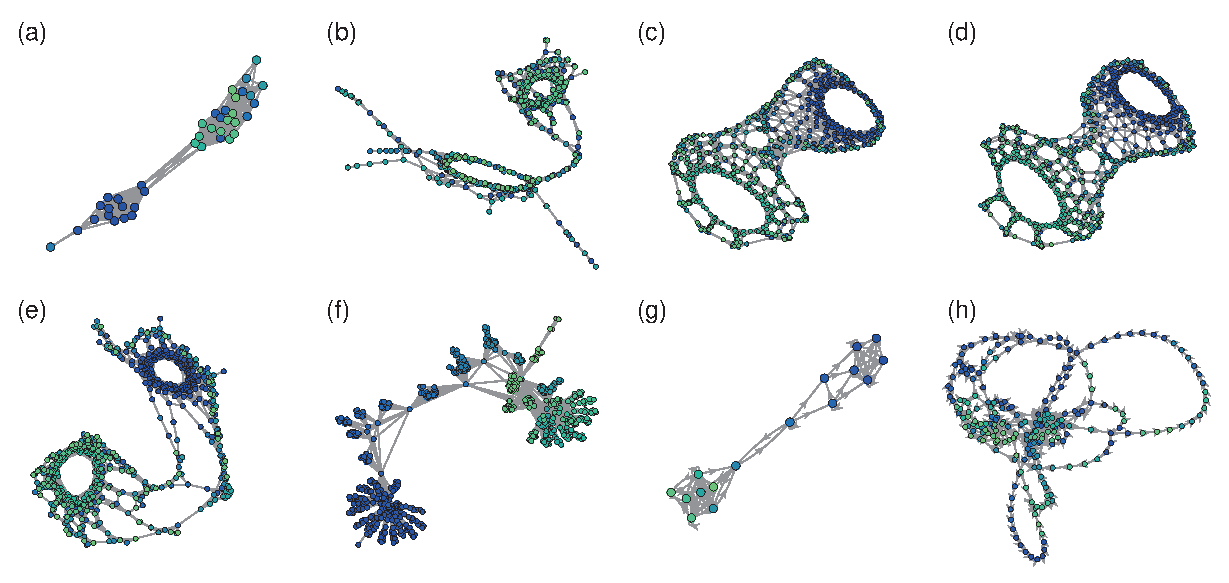
\includegraphics[width=\textwidth]{Chapter01_Introduction/lorenz_network.eps} 
\caption{Graphical representation of the different complex networks based on the adjacency matrices shown in Fig.~\ref{fig:lorenz_adj-matrices}. The graphs have been embedded into an abstract two-dimensional space using a force directed placement algorithm~\cite{Battista1994}, which has been integrated into the {\tt {graph}} toolbox of Matlab. For panels (a)-(f), the vertex color indicates the temporal order of observations (from blue to green), for transition networks (panels (g, h)), colors correspond to the different partitions. Note that in panels (b), (g) and (h) some individual disconnected vertices have been removed from the corresponding network representations. Modified from \cite{Donner2011}. } \label{fig:lorenz_network}
\end{figure}

    In this review we provide in-depth discussions on complex network representations of individual or potentially interrelated time series, which distinctively differ from existing dara minimg tools from computer sciences \cite{Zanin2016} as discussed above in terms of the underlying motivation and methodology. Specifically, all network approaches discussed in this report provide different applications of complex network theory to nonlinear time series analysis. We do not further expand the discussion on the differences between time series networks and data mining tools to keep this report topically focused.

	\subsection{Transformations of time series into the complex network domain}
	In order to make time series accessible to complex network analysis techniques, we have to transform them into a proper network representation. At a first place, this requires an algorithm defining network vertices and edges. Depending on these definitions, there are at least three main classes of complex network approaches to the analysis of individual time series that will be put in the focus of this review (see Tab.~\ref{tab:methods}). These three types of methods are based on different rationales, i.e.,
\begin{enumerate}[(i)]
\item mutual statistical similarity or metric proximity between different segments of a time series (proximity networks),
\item convexity of successive observations (visibility graphs), and
\item transition probabilities between discrete states (transition networks).
\end{enumerate}

	The first important class of time series networks make use of similarities or proximity relationships between different parts of a dynamical system's trajectory \cite{Marwan2009,Donner2010a,Donner2011}, including such diverse approaches as cycle networks \cite{Zhang2006,Zhang2008e}, correlation networks \cite{Yang2008}, and phase space networks based on a certain definition of nearest neighbors \cite{Xu2008}. One especially important example of proximity networks are recurrence networks (RNs) \cite{Marwan2009,Donner2010a}, which provide a reinterpretation of recurrence plots \cite{marwan2007} in network-theoretic terms and are meanwhile widely applied in a variety of fields. 

	The second class are visibility graphs and related concepts, which characterize some local convexity or record-breaking property within univariate time series data \cite{Lacasa2008,Luque2009,Donner2012}. The standard visibility graph and its various variants have important applications, such as providing new estimates of the Hurst exponent of fractal and multi-fractal stochastic processes \cite{Lacasa2009,Ni2009} or statistical tests for time series irreversibility \cite{Donges2013,Lacasa2012}. 

	The third important class of network approaches are transition networks, which make use of ideas from symbolic dynamics and stochastic processes. Transforming a given time series into a transition network is a process of mapping the temporal information into a Markov chain to obtain a compressed or simplified representation of the original dynamics. More specifically, we first discretize the dynamics and then study the transition probabilities between the obtained groups in some Markov chain-like ways \cite{Nicolis2005}. Depending on the particular choice of partitions, we obtain different versions of transition networks. For instance, we can construct transition networks by threshold-based coarse graining of the underlying system's phase space \cite{Donner2011} or based on ordinal patterns \cite{McCullough2015,Kulp2016b}. 

	It may be interesting to note that both, proximity networks and transition networks, are somewhat related with the concept of recurrence in one way or the other \cite{Donner2011}. This is particularly evident for proximity networks, where connectivity is defined in a data-adaptive local way, i.e., by considering distinct regions with a varying center at a given vertex in either the phase space itself or an abstract metric space where (pseudo) distances measure similarities between states or sequences thereof. In contrast, for transition networks, the corresponding classes are rigid, i.e., determined by a fixed coarse-graining of the phase space, ordinal patterns, or other related symbolic approaches. In this regard, the distinction between both classes of time series network approaches closely resembles the duality between phase space based approaches of nonlinear time series analysis on the one hand, and symbolic time series analysis and related information-theoretic approaches, which may both be used for estimating similar dynamical invariants such as entropies and mutual information \cite{Balasis2013}.
\begin{table}[t]
\caption{Summary of the definitions of vertices and the criteria for the existence of edges in existing complex network approaches.}{
\resizebox{\columnwidth}{!}{%
\begin{tabular}{llll}
\hline
Method & Vertex & Edge & Directedness \\
\hline
Proximity networks & & \\
\textit{Cycle networks} & Cycle & Correlation or phase space distance between cycles & undirected \\
\textit{Correlation networks} & State vector & Correlation coefficient between state vectors & undirected \\
\textit{Recurrence networks} & & & \\
\quad \textit{$k$-nearest neighbor networks}& State (vector) & Recurrence of states (fixed neighborhood mass) & directed \\
\quad \textit{adaptive nearest neighbor networks}& State (vector)  & Recurrence of states (fixed number of edges) & undirected \\
\quad \textit{$\varepsilon$-recurrence networks} & State (vector) & Recurrence of states (fixed neighborhood volume) & undirected \\
\hline
Visibility graphs &  &  &  \\
\quad \textit{natural visibility graphs}& Scalar state & Mutual visibility of states & undirected \\
\quad \textit{horizontal visibility graphs}& Scalar state  & Horizontal mutual visibility of states & undirected \\
\hline
Transition networks &  &  &  \\
\quad \textit{threshold based networks}& Phase space partition & Temporal succession & directed \\
\quad \textit{ordinal pattern networks}& Ordinal patterns  & Temporal succession & directed \\
\hline
\end{tabular}
}
\normalsize
\label{tab:methods}}
\end{table}

	Among the three classes of methods listed above, the largest group of concepts is given by proximity networks, where the mutual closeness or similarity of different segments of a trajectory can be characterized in different ways. Consequently, there are various types of such proximity networks (see Tab.~\ref{tab:methods}). However, all these methods are characterized by two common general properties: Firstly, the resulting networks are invariant under relabeling of their vertices in the adjacency matrix. Hence, the topological characteristics of proximity networks yield nonlinear measures that are invariant under a permutation of their vertices. In this respect, these network-theoretic approaches are distinctively different from traditional methods of time series analysis where the temporal order of observations does explicitly matter. Secondly, we point out that especially proximity networks are spatial networks \cite{Barthelemy2011,Wiedermann2016}. In particular, recurrence networks are embedded in the phase space of the considered system, with distances being defined by one of the standard metrics (e.g., Euclidean, Manhattan, etc.), making them a specific type of random geometric graphs \cite{Donner2011b}. Similar considerations apply to other types of proximity networks as well. Moreover, also visibility graphs and related concepts can be viewed as spatially embedded networks, for which the one-dimensional time axis takes the role of a metric space in which the resulting network's vertices and edges are embedded.

\subsection{Outline of the report}
The remainder of this review is organized as follows: 

In Section \ref{sec:CompNetworkT}, we start with a brief introduction on complex network theory, mainly focusing on the characterization of the structural properties of networks based on the adjacency matrix. All relevant terminologies of network measures will be introduced in this section. We also discuss some concepts that are particularly important for transforming time series into network representations, particularly, the definitions of network vertices and edges. 

In Section \ref{sec:RecurrenceNt}, we focus on recurrence network approaches (RN). We will cover the theoretical background of Poincar\'e recurrences in dynamical systems and the popular visualization technique of recurrence plots \cite{marwan2007}. Furthermore, we summarize the current state of knowledge on the theoretical foundations and potential applications of RN approaches to nonlinear time series. We demonstrate that this type of time series networks naturally arise as random geometric graphs in the phase space of dynamical systems, which determines their structural characteristics and gives rise to a dimensionality interpretation of clustering coefficients and related concepts. Beyond the single-system case, we also provide a corresponding in-depth discussion of cross- and joint recurrence plots from the complex network viewpoint. Moreover, we discuss some recent ideas related to the utilization of multiplex and multilayer multivariate recurrence network-based approaches for studying geometric signatures of coupling and synchronization processes. 

In Section \ref{sec:VisibilityGt}, both the standard visibility graphs (VG) and horizontal visibility graphs (HVG) will be reviewed. We start with discussing the main variants of visibility algorithms applied in the context of time series analysis. Specifically, we summarize some conjectures of theoretical predictions of (H)VG properties in stochastic and deterministic processes. Some practical considerations when applying (H)VG analysis to experimental time series will be thoroughly discussed. In addition, we will discuss the generalization of (H)VG analysis from univariate to bi- and multivariate time series, for instance, multiplex (H)VGs. We further show that a decomposition of (H)VGs into time forward (outgoing) and backward (incoming) directions helps to test irreversibility of the underlying time series. 

In Section \ref{sec:TransitionNt}, we introduce the construction of transition networks by proper coarse graining of phase space and ordinal patterns. Specifically, the concept of ordinal pattern transition networks can be traced back to identifying ordinal patterns of time series \cite{Bandt2002}. We particularly review the ordinal pattern transition networks of \cite{McCullough2015} and their generalizations to multivariate time series \cite{Zhang2017b}, highlighting their great potential for studies of experimental observation data from climate sciences \cite{Eroglu2016}. 

In Section \ref{sec:Applications}, we review several applications of network approaches to different real-world time series. The following Section \ref{sec:Software} briefly summarizes existing software implementations, with a particular focus on the Python package \texttt{pyunicorn} that includes several methods from both, complex network theory and nonlinear time series analysis, including several of the approaches discussed in this review, and unites them in a high-performance, modular and flexible way \cite{Donges2015}. Finally, Section \ref{sec:Discussion} summarizes the main topics addressed in this report and puts them into a broader perspective. Specifically, we will outline a few important general directions for future research. We emphasize that applying complex network methods for time series analysis is still an emerging field, and that there are numerous relevant topics from both the theoretical and applied perspectives that still deserve further exploration.


